\documentclass{beamer}


\usepackage{amsmath}
\usepackage[style=alphabetic,url=true]{biblatex}
\usepackage{environ}
\usepackage{geometry}
\usepackage{graphicx}
\usepackage{tikz}
\usepackage[T2A]{fontenc}
\usepackage[utf8]{inputenc}
\usepackage[cache=false]{minted}
\usepackage{amsmath}
\usepackage{amsfonts}
\usepackage{amssymb}
\usepackage{calrsfs}


% \usetheme{Bergen}

\usecolortheme{beaver}

\setbeamertemplate{itemize item}[circle]
\setbeamertemplate{itemize subitem}{--}
\addtobeamertemplate{navigation symbols}{}{
  \usebeamerfont{footline}%
  \usebeamercolor[fg]{footline}%
  \hspace{1em}%
  \insertframenumber/\inserttotalframenumber
}
\graphicspath{ {./graphics/} }
\setminted[Python]{
  fontsize=\tiny
}
\BeforeBeginEnvironment{minted}{\medskip}
\AfterEndEnvironment{minted}{\medskip}



\title{
  Біткоїн та криптовалютні технології \\
  Лекція 2: Основи криптографії 1/2
}

\author{Юрій Жикін}
\date{28 вересня, 2022}

\begin{document}

\frame{\titlepage}

\begin{frame}
  \frametitle{Вступ до криптографії 1/2}
  \begin{itemize}
  \item \textbf{Криптографія} (з дав. грецької, ``прихований, таємний'' і
    ``писати'') - теорія і практика технік \textit{безпечної комунікації} в
    умовах присутності \textit{присутності \textbf{зовнішнього спостерігача},
      якого називають ворогом (супротивником)}.
  \item \textbf{Сучасна криптографія} майже повністю базується на
    \textit{математичній теорії і комп'ютерних науках}.
  \item \textbf{Сучасні криптографічні алгоритми} базуються на припущення про
    обчислювальну складність деяких задач.
  \end{itemize}
\end{frame}

\begin{frame}
  \frametitle{Вступ до криптографії 2/2}
  \begin{itemize}
  \item Сучасна криптографія поділяється на дві категорії:
    \begin{itemize}
    \item \textbf{симетрична криптографія} - обидві сторони мають спільний
      секретний ключ, який використовується для шифрування та дешифрування,
    \item \textbf{несиметрична криптографія (криптографія з публічним, або
        відкритим, ключем)} - ключ складається з публічної, або відкритої, та
      приватної, або закритою, частин; публічний ключ використовується для
      шифрування, а приватний ключ - для дешифрування.
    \end{itemize}
  \item Криптографічні протоколи виконують для двох основних цілей:
    \begin{itemize}
    \item \textbf{приховування інформації} (шифрування/дешифрування),
    \item \textbf{забезпечення цілісності інформації} (цифрові підписи і їх
      верифікації).
    \end{itemize}
  \end{itemize}
\end{frame}

\begin{frame}
  \frametitle{Симетрична криптографія}
  \begin{itemize}
  \item Єдиний вид криптографії до 1976 року.
  \item Обидві сторони мають спільний таємний ключ, який використовується для
    шифрування та дешифрування.
  \item Алгоритми симетричного шифрування дуже швидкі (наприклад \textit{AES},
    \textit{Salsa20}, \textit{ChaCha}).
  \item Більшість популярних алгоритмів симетричного шифрування реалізовано ``в залізі''
    (наприклад \textit{AES} та AES-NI інструкції в процесорах архітектури x86).
  \item Схема досконалого шифрування:
    \begin{align*}
      &E = M \oplus K, \\
      &D = E \oplus K, \\
      &|M| == |K|
    \end{align*}
  \end{itemize}
\end{frame}

\begin{frame}
  \frametitle{Недоліки симетричної криптографії}
  \begin{itemize}
  \item Сторони повинні заздалегідь домовитись про таємний ключ через безпечний
    канал зв'язку - проблема ``курки та яйця''.
  \item Симетричність витоку - якщо стається витік ключа у однієї з сторін,
    обидві сторони скомпрометовано.
  \item Якщо декілька сторін мають один спільний ключ, симетрія витоку зачіпає
    всіх учасників.
  \item Якщо кожен з учасників має окремий ключ для кожного іншого учасника в
    системі, виникає проблема зберігання ключів.
  \end{itemize}
\end{frame}

\begin{frame}
  \frametitle{Асиметрична криптографія}
  \begin{itemize}
  \item Фундаментальне відкриття \textbf{Вітфілда Діффі}, \textbf{Мартіна
      Гелмана} та \textbf{Ральфа Меркла} у 1976 році.
  \item Повідомлення шифруються публічним (відкритим) ключем, але можуть бути
    дешифровані лише приватним (закритим) ключем.
  \item Кожна сторона відповідальна лише за зберігання власного приватного ключа
    - публічний ключ може бути обчислений з приватного ключа, і може бути
    надісланий через будь-який незахищений канал зв'язку.
  \end{itemize}
\end{frame}

\begin{frame}[fragile]
  \frametitle{Ймовірнійсть та випадкові великі числа 1/4}
  \begin{itemize}
  \item В більшості сучасних криптографічних систем безпека ключа базується на
    ймовірності вгадування дуже великого числа.
  \item Для того, щоб зробити вгадування ключа якомога складнішим, числа повинні
    бути справді випадковими: ймовірнійсть того, що кожен біт в числі є 1 чи 0,
    повинна бути рівною 0.5.
  \item Ймовірність вгадування дійсно випадкового числа $N$ становить $1/N$.
  \item Приблизна оцінка кількості атомів у Всесвіті становить $10^{78} \simeq
    2^{259}$, отже вгадування 256-бітного ключа можна порівняти з вгадуванням
    конкретного атома у Всесвіті.
  \end{itemize}
\end{frame}

\begin{frame}[fragile]
  \frametitle{Ймовірність та випадкові великі числа 2/4}
  \begin{itemize}
  \item В той же час, великі числа, що використовуються як криптографічні ключі,
    можуть бути компактно представлені у 16-ковому чи 64-ковому кодуванні:
\begin{minted}{Python}
import secrets
import base64
bits = secrets.randbits(256)
# 46518555179467323509970270980993648640987722172281263586388328188640792550961
bits_binary = '{0:b}'.format(bits)
# 110011011011000100100011011010111101101011111110101000111100101000001000100101\
# 111100110101001111110101111100100111000101110101011100011001010111001011000001\
# 111010110101010000010001000001111110111110011000000110011100100111111010110100\
# 100100001111000110001
bits_hex = hex(bits)
# 0x66d891b5ed7f51e5044be6a7ebe4e2eae32b960f5aa0883f7cc0ce4fd6921e31
bits_base64 = base64.b64encode(bits.to_bytes(32, 'little'))
# MR6S1k/OwHw/iKBaD5Yr4+ri5Oun5ksE5VF/7bWR2GY=
\end{minted}
  \end{itemize}
\end{frame}

\begin{frame}[fragile]
  \frametitle{Ймовірність та випадкові великі числа 3/4}
  \begin{itemize}
  \item Комп'ютери детерміністичні, тому генерація дійсно випадкових чисел - це
    нетривіальна задача.
  \item В більшості випадків, найбільш безпечний спосіб отримати випадкове число
    в Unix-подібних операційних системах - це прочитати послідовність байтів з
    віртуального пристрою \mintinline{Bash}{/dev/random} чи
    \mintinline{Bash}{/dev/urandom}.
  \item Існують спеціальні пристрої, які генерують дійсно випадкові числа на
    основі ентропії середовища; якщо це можливо, варто віддавати їм перевагу для
    генерацї криптографічних ключів.
  \end{itemize}
\end{frame}

\begin{frame}[fragile]
  \frametitle{Ймовірнійсть та випадкові великі числа 4/4}
  \begin{itemize}
  \item Люди дуже погано вміють сприймають дісно випадкові величини через те, що
    вони мають еволюційно гіпертрофовану здатність знаходити закономірності.
    \begin{center}
      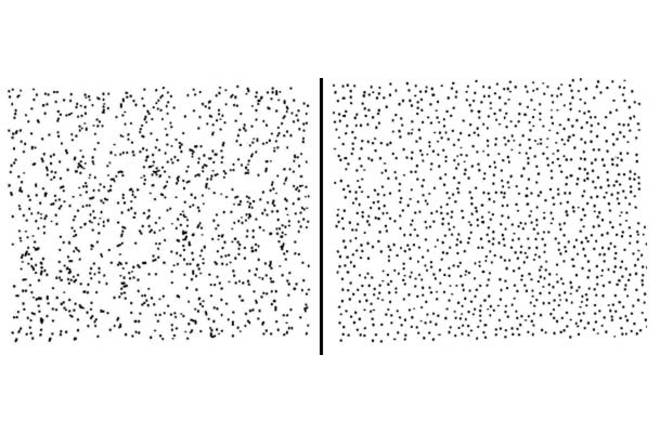
\includegraphics[width=0.9\textwidth,]{random_dots}
    \end{center}
  \end{itemize}
\end{frame}

\begin{frame}
  \frametitle{Хеш-функції}
  \begin{itemize}
  \item \textbf{Хеш-функція} - це функція, що перетворює значення довільного
    розміру у значення фіксованого розміру.
  \item Хеш-функції використовуються для адресації у структурах даних (хеш-таблиці),
    ймовірнісних фільтрах (фільтри Блума), тощо.
    \begin{center}
      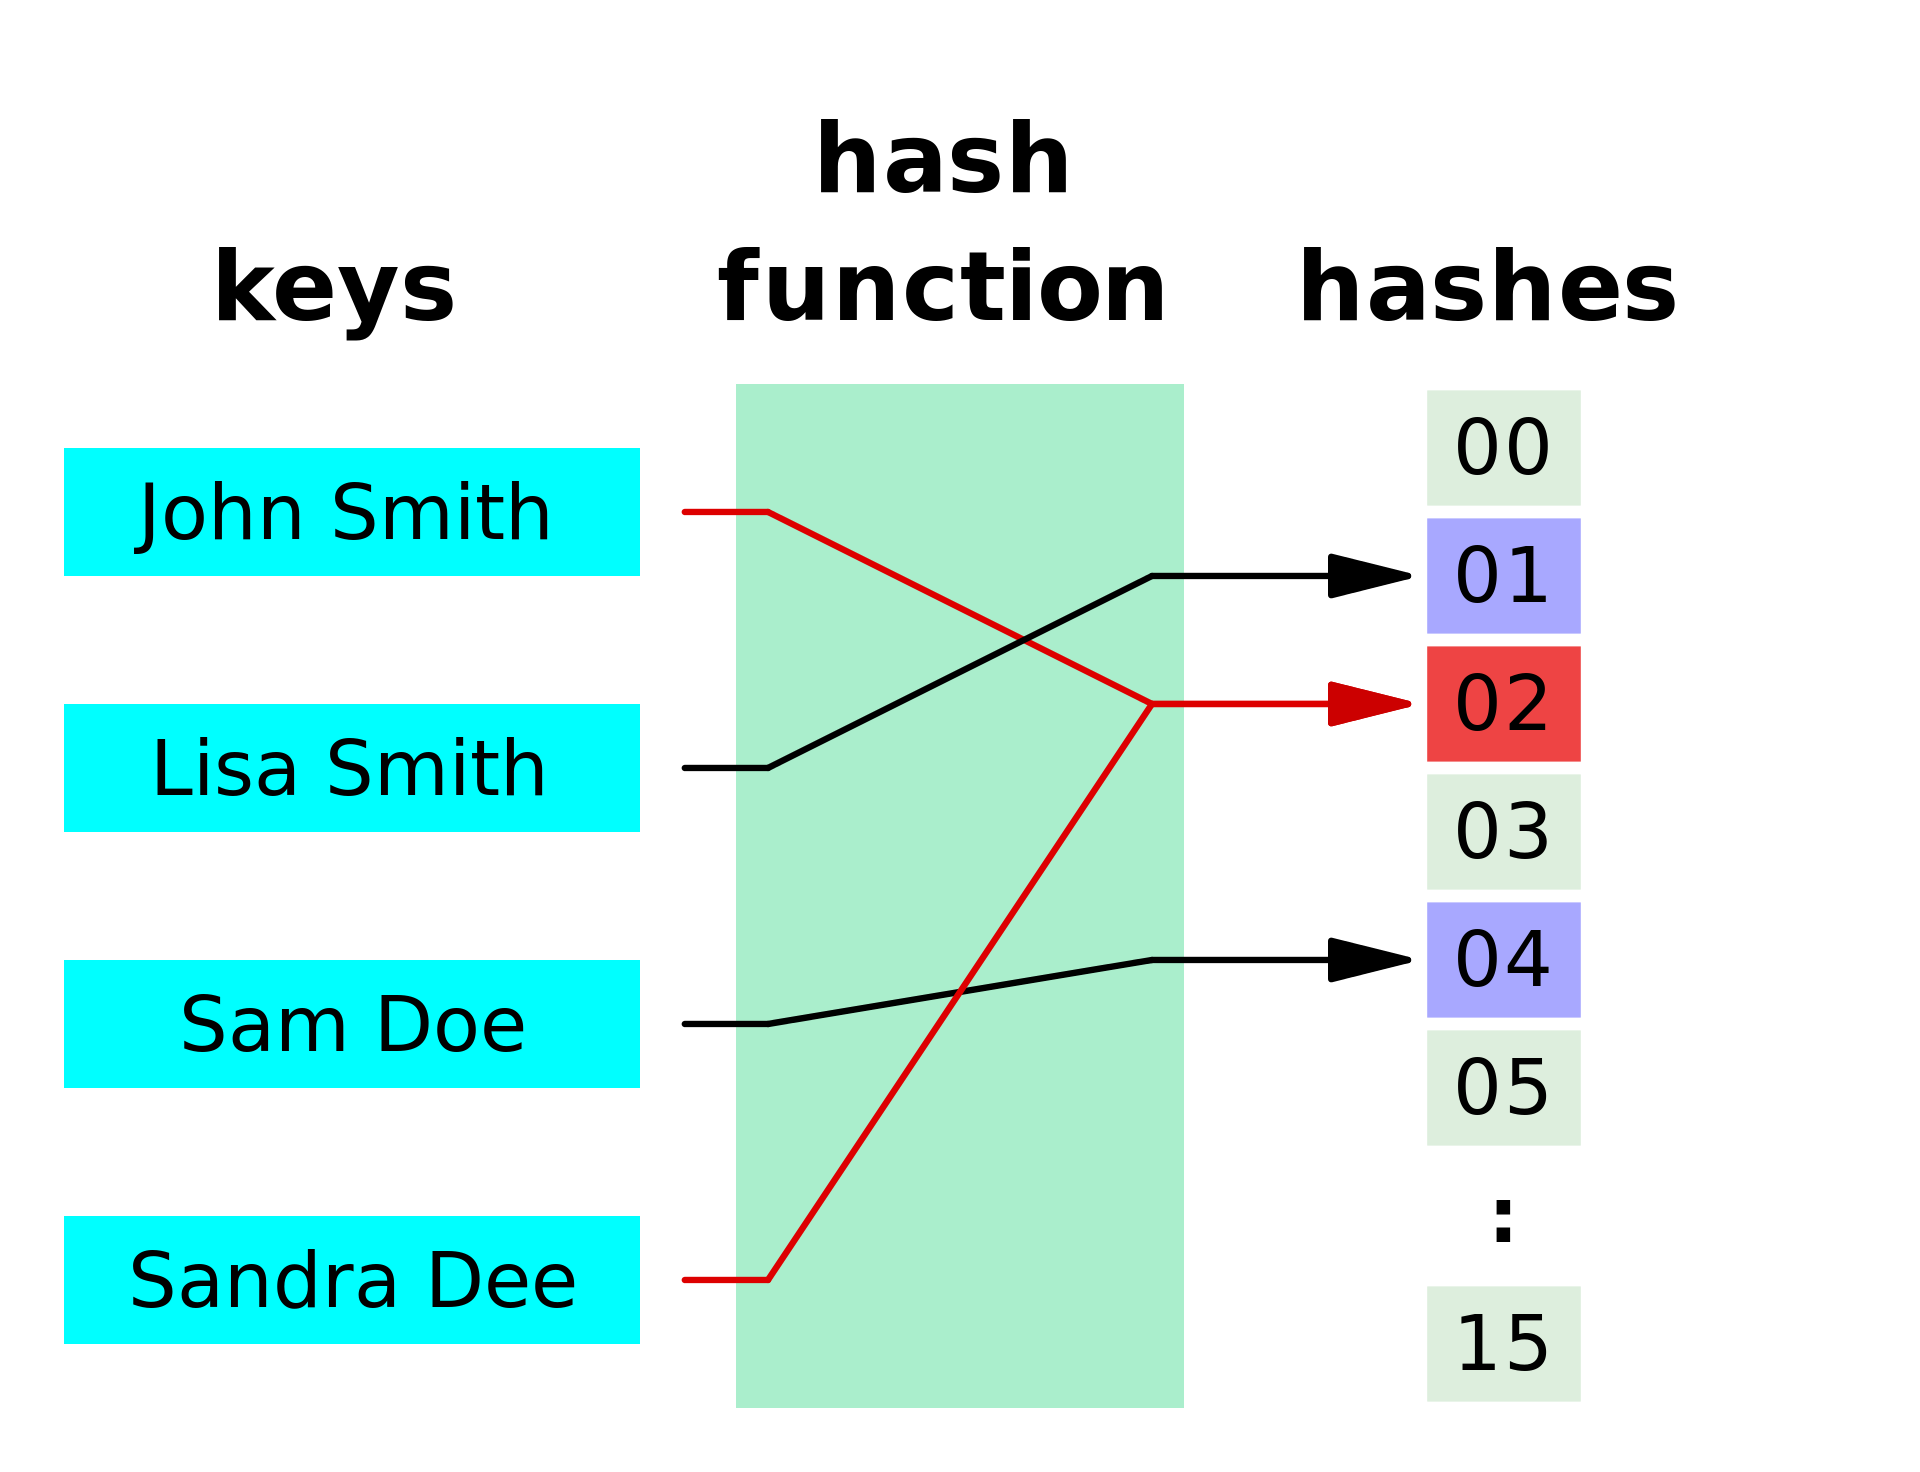
\includegraphics[width=0.6\textwidth,]{hash_function}
    \end{center}
  \end{itemize}
\end{frame}

\begin{frame}
  \frametitle{Криптографічні хеш-функції}
  \begin{itemize}    
  \item \textbf{Криптографічні хеш-функції} - це \textit{хеш-функції}, що
    перетворюють довільні дані у послідовності бітів фіксованого розміру і є
    \textbf{односторонніми функціями}, тобто функціями, які практично неможливо
    інвертувати:
    \begin{align*}
      h = H(m)&\text{ - ефективно,}\\
      m = H^{-1}(h)&\text{ - \textbf{дуже} неефективно}
    \end{align*}
  \item \textbf{Найбільш ефективними} способом інвертувати криптографічну
    хеш-функцію, тобто знайти вхідне повідомлення $m$ такі, що перетворюються у хеш $h$
    даною хеш-функцією, - це пошук ``грубою силою'', або повний перебір, -
    обираємо випадкове повідомлення $m_i$ і перевіряємо, чи $H(m_i) = h$.
  \item Фундаментальний інструмент сучасної криптографії.
  \end{itemize}
\end{frame}

\begin{frame}
  \frametitle{Властивості криптографічних хеш-функцій 1/2}
  \begin{itemize}
  \item Основні властивості \textbf{надійних} криптографічних хеш-функцій:
    \begin{itemize}
    \item \textbf{детермінізм} - той же вхід завжди дає той же вихід (хеш),
    \item \textbf{ефективність} - хеш даного повідомлення можна обчислити дуже швидко,
    \item \textbf{дифузія, ``лавинна властивість} - зміна одного біта у
      повідомленні $m$ призводить до зміни кожного біта у $h$ з ймовірністю 0.5,
    \item \textbf{стійкість до пошуку прообразу} - маючи хеш $h$, повинно бути
      складно знайти будь-яке повідомлення $m$ таке, що $h = H(m)$,
    \item \textbf{стійкість до пошуку другого прообразу} - маючи повідомлення
      $m_1$, повинно бути складно знайти будь-яке повідомлення $m_2$ таке, що
      $H(m_1) = H(m_2)$,
    \item \textbf{стійкість до колізій} - повинно бути складно знайти будь-які
      два повідомлення $m_1$ і $m_2$ такі, що $H(m_1) = H(m_2)$.
    \end{itemize}
  \end{itemize}
\end{frame}

\begin{frame}
  \frametitle{Властивості криптографічних хеш-функцій 2/2}
  \begin{itemize}
  \item Додаткові властивості \textbf{надійних} криптографічних хеш-функцій:
    \begin{itemize}
    \item \textbf{стійкість до збільшення довжини} - маючи $h = H(m)$ і
      $len(m)$, повинно бути складно знайти $h' = H(m || m')$,
    \item \textbf{сильна стійкість до колізій} - стійкість до атак через
      \textbf{парадокс днів народження}.
      resistance.
    \end{itemize}
  \end{itemize}
\end{frame}

\begin{frame}
  \frametitle{Використання криптографічних хеш-функцій 1/2}
  \begin{itemize}
  \item \textbf{Коди аутентифікації повідомлень (MAC)} - хеш якогось
    повідомлення, поєднаного з якимось ключем, дозволяє перевірити цілісність
    даного повідомлення.
  \item \textbf{Цифрові підписи} - підписування хеша повідомлення є значно більш
    швидкою операцією, ніж підписування цілого повідомлення.
  \item \textbf{Перевірка паролів} - зберігання паролів у відкритому вигляді
    призводить до серйозних порушень безпеки, якщо база даних з паролями ``витікає''
    назовні; зберігання хешів паролів дозволяє цього уникнути.
  \item \textbf{Сильні перевірки цілісності даних (чек-суми)} - використовуються
    замість звичайних некриптографічних хеш-функцій, коли необхідні більш
    надійні гарантії.
  \item Приклади: \textbf{SHA-2} (\textbf{SHA-256}, \textbf{SHA-512}),
    \textbf{RIPEMD-160}, \textbf{SHA-3}.
  \end{itemize}
\end{frame}

\begin{frame}
  \frametitle{Використання криптографічних хеш-функцій 2/2}
  \begin{itemize}
  \item \textbf{Докази виконаної роботи (Proof-of-Work)} - основа сучасних
    криптовалютних технологій.
  \item \textit{Hashcash} - оригінальна ідея, запропонована Адамом Беком у 1997
    році як засіб боротьби з спамом в системах електронної пошти та атаками
    відмови в обслуговуванні.
  \item Основна ідея \textbf{PoW}:
    \begin{itemize}
    \item для деякого повідомлення $m$, виконуємо \textbf{пошук шляхом ``грубої
        сили''} значенн $r$ такого, що $h = H(m, r)$ задовільняє певний
      критерій, наприклад 
      \begin{align*}
        h < h_{target}
      \end{align*}
    \item критерій пошуку може бути обрано таким, що пошук значення $r$ за
      допомогою якоїсь обчислювальної потужності займатиме в середньому певну
      кількість часу.
    \end{itemize}
  \item Обчислення \textbf{доказу виконаної роботи} потребує конкретної
    кількості енергії, яку можна оцінити, і ця кількість може бути достатно
    великою, щоб обчислення нового доказу було дорогим.
  \end{itemize}
\end{frame}

\begin{frame}
  \frametitle{Корисні ресурси}
  \begin{itemize}
  \item Dan Boneh's Cryptography I course from Stanford University -
    https://www.coursera.org/learn/crypto.
  \item Serious Cryptography: A Practical Introduction to Modern Encryption -
    Jean-Philippe Aumasson.
  \item 8 sets of cryptography problems that introduce various real-life
    cryptography systems and show practical attacks on them -
    https://cryptopals.com.
  \end{itemize}
\end{frame}

\begin{frame}
  \frametitle{Кінець}
  \begin{center}
    Дякую за увагу!
  \end{center}
\end{frame}

\end{document}

%%% Local Variables:
%%% mode: latex
%%% TeX-master: t
%%% End:
